\documentclass{beamer}

\usefonttheme{professionalfonts} % using non standard fonts for beamer
\usefonttheme{serif} % default family is serif

%\usepackage{hyperref}

%\usepackage{minted}

\usepackage{animate}

\usepackage{graphicx}

\def\Put(#1,#2)#3{\leavevmode\makebox(0,0){\put(#1,#2){#3}}}

\usepackage{color}

\usepackage{tikz}

\usepackage{amssymb}

\usepackage{enumerate}


\newcommand\blfootnote[1]{%

  \begingroup

  \renewcommand\thefootnote{}\footnote{#1}%

  \addtocounter{footnote}{-1}%

  \endgroup

}

\makeatletter

%%%%%%%%%%%%%%%%%%%%%%%%%%%%%% Textclass specific LaTeX commands.

 % this default might be overridden by plain title style

 \newcommand\makebeamertitle{\frame{\maketitle}}%

 % (ERT) argument for the TOC

 \AtBeginDocument{%

   \let\origtableofcontents=\tableofcontents

   \def\tableofcontents{\@ifnextchar[{\origtableofcontents}{\gobbletableofcontents}}

   \def\gobbletableofcontents#1{\origtableofcontents}

 }

%%%%%%%%%%%%%%%%%%%%%%%%%%%%%% User specified LaTeX commands.

\usetheme{Malmoe}

% or ...

\useoutertheme{infolines}

\addtobeamertemplate{headline}{}{\vskip2pt}



\setbeamercovered{transparent}

% or whatever (possibly just delete it)

\makeatother

\begin{document}
\title[DDCEL report]{A Scalable DCEL implementation}
\author[AC]{Andres Calderon}
\institute[Spring'20]{University of California, Riverside}
\makebeamertitle
\newif\iflattersubsect

\AtBeginSection[] {
  \begin{frame}<beamer>
    \frametitle{Outline} 
    \tableofcontents[currentsection]  
  \end{frame}
  \lattersubsectfalse
}

\AtBeginSubsection[] {
  \begin{frame}<beamer>
    \frametitle{Outline} 
    \tableofcontents[currentsubsection]  
  \end{frame}
}

\begin{frame}{Experiment settings}
    \begin{itemize}
     \item California district dataset (2000 and 2010) Dataset
     \item 12 Nodes 8 Cores each
     \item Variying number of partitions
     \item Average of 10 runs
    \end{itemize}
\end{frame}
\begin{frame}{Experiment results}{General}
    \centering
	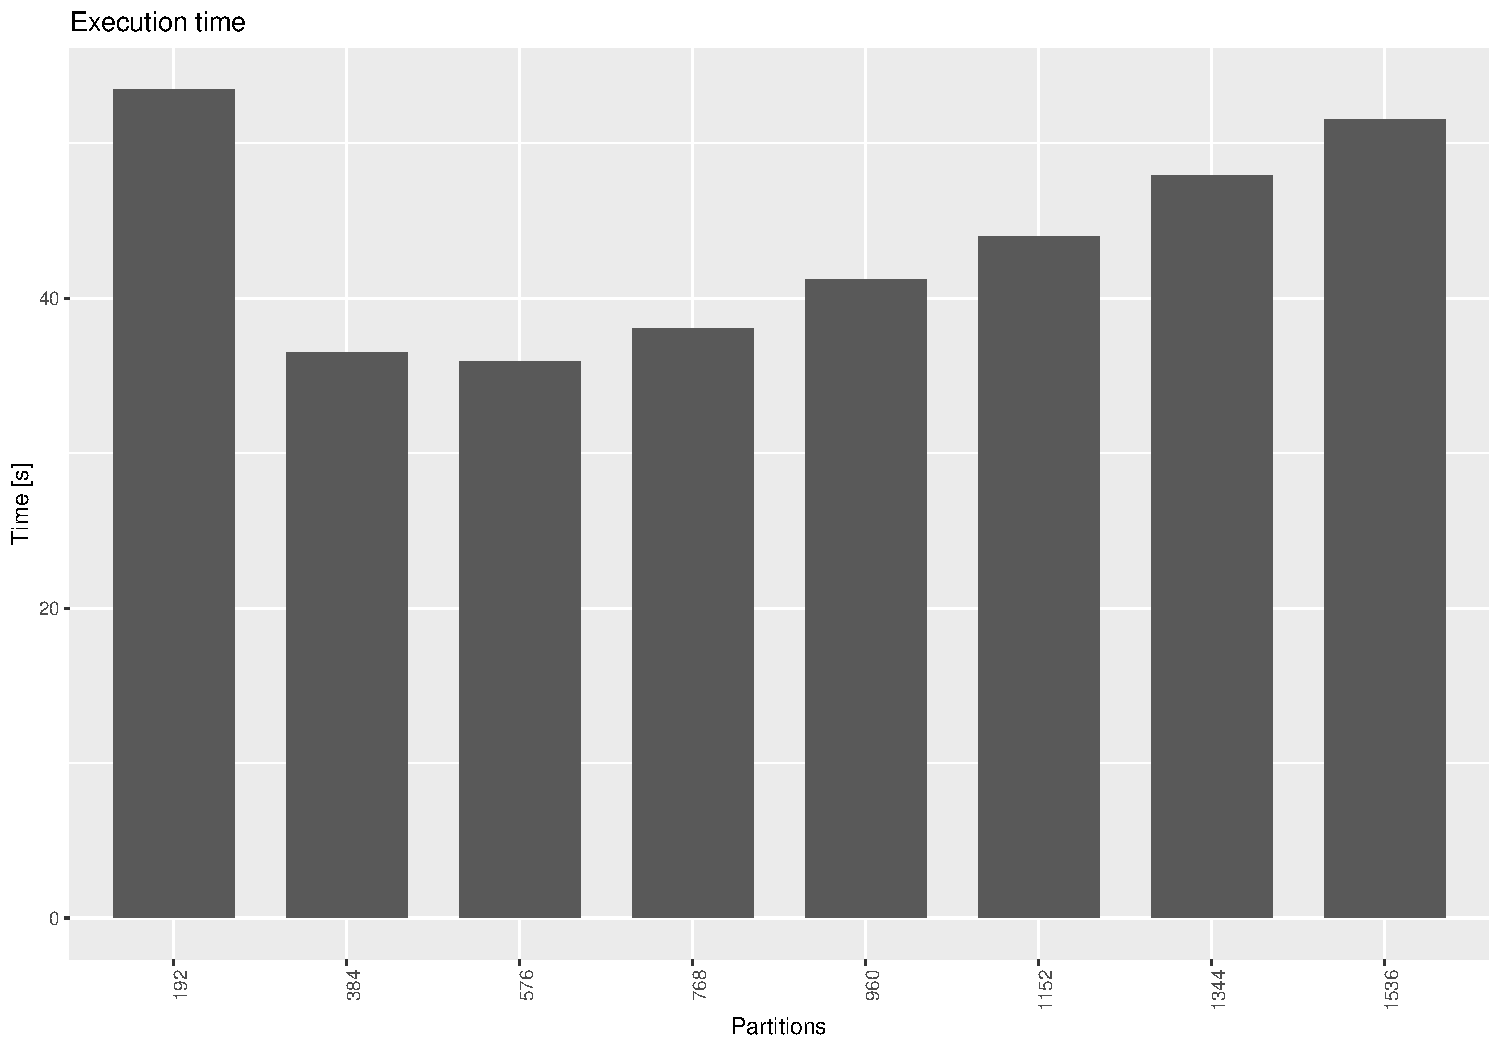
\includegraphics[width=0.8\textwidth]{figures/ByPartitions}
\end{frame}
\begin{frame}{Experiment results}{By stages}
    \centering
	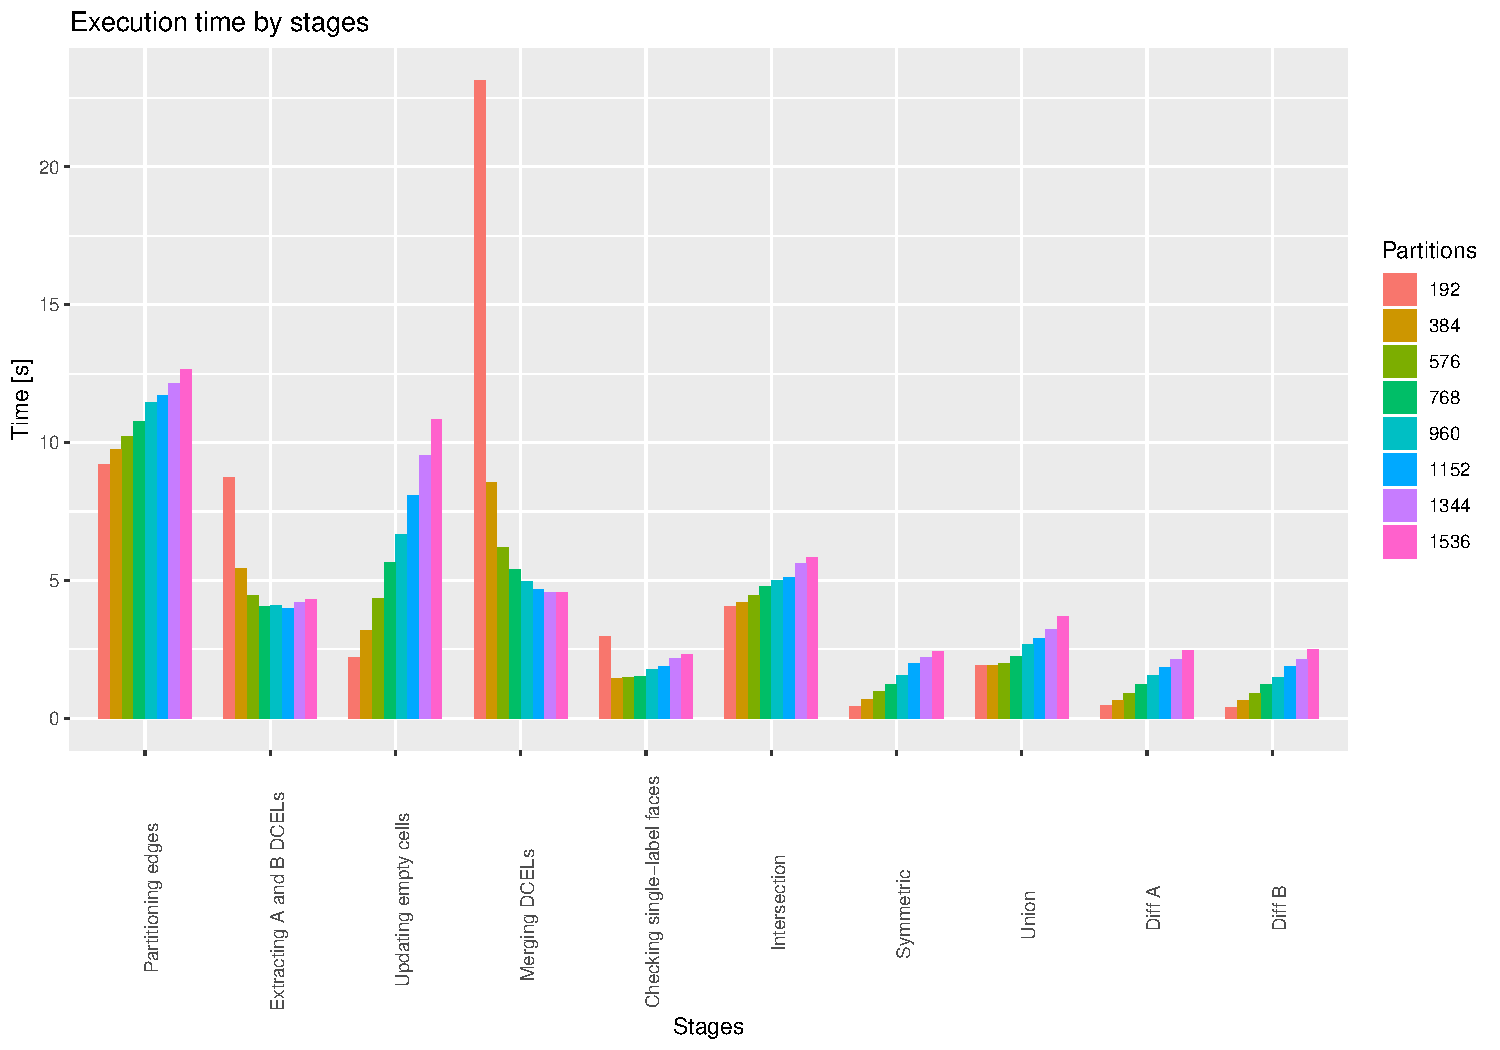
\includegraphics[width=0.8\textwidth]{figures/ByStages}
\end{frame}

\begin{frame}{Traking task balance in the cluster}
    \centering
	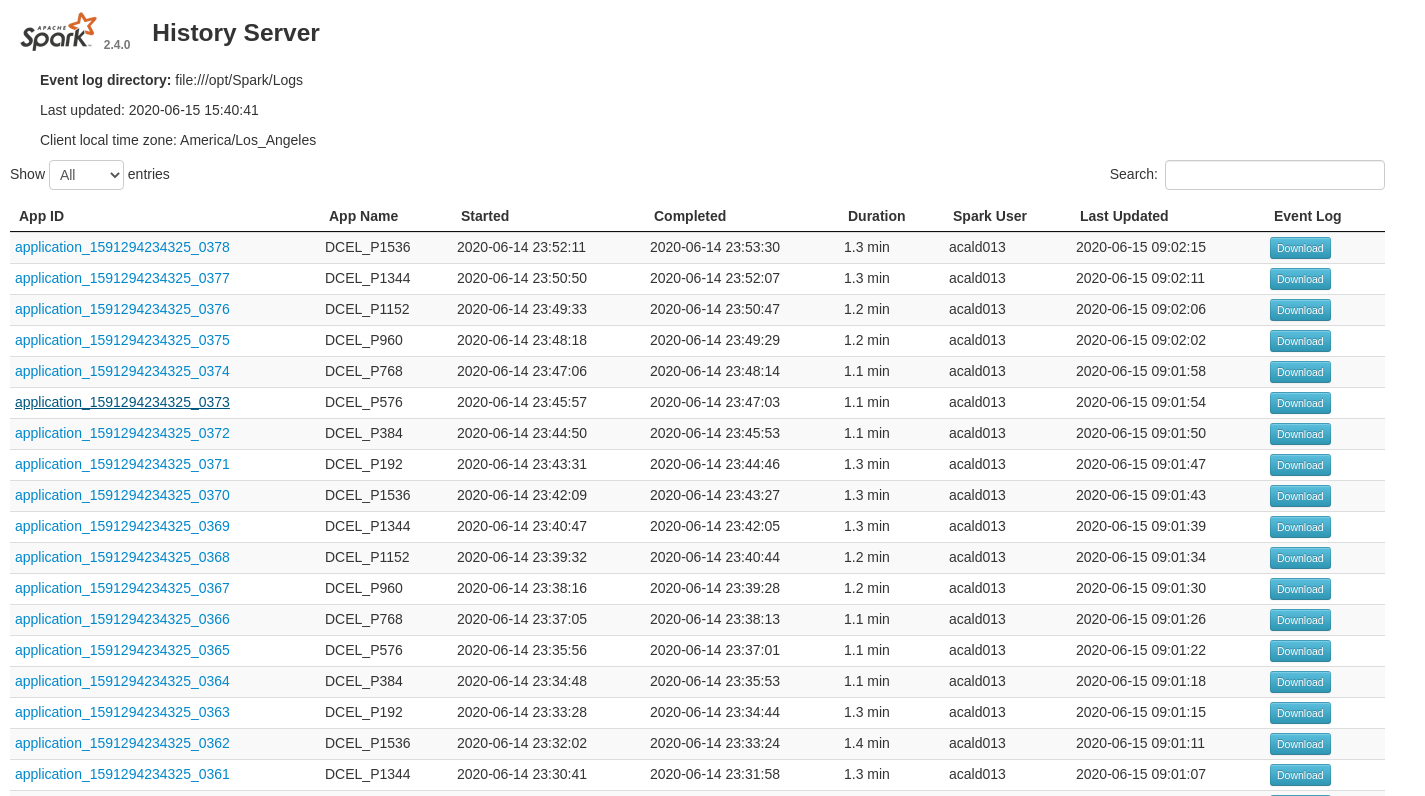
\includegraphics[width=1\textwidth]{figures/apps}
\end{frame}

\begin{frame}{Traking task balance in the cluster}
    \centering
	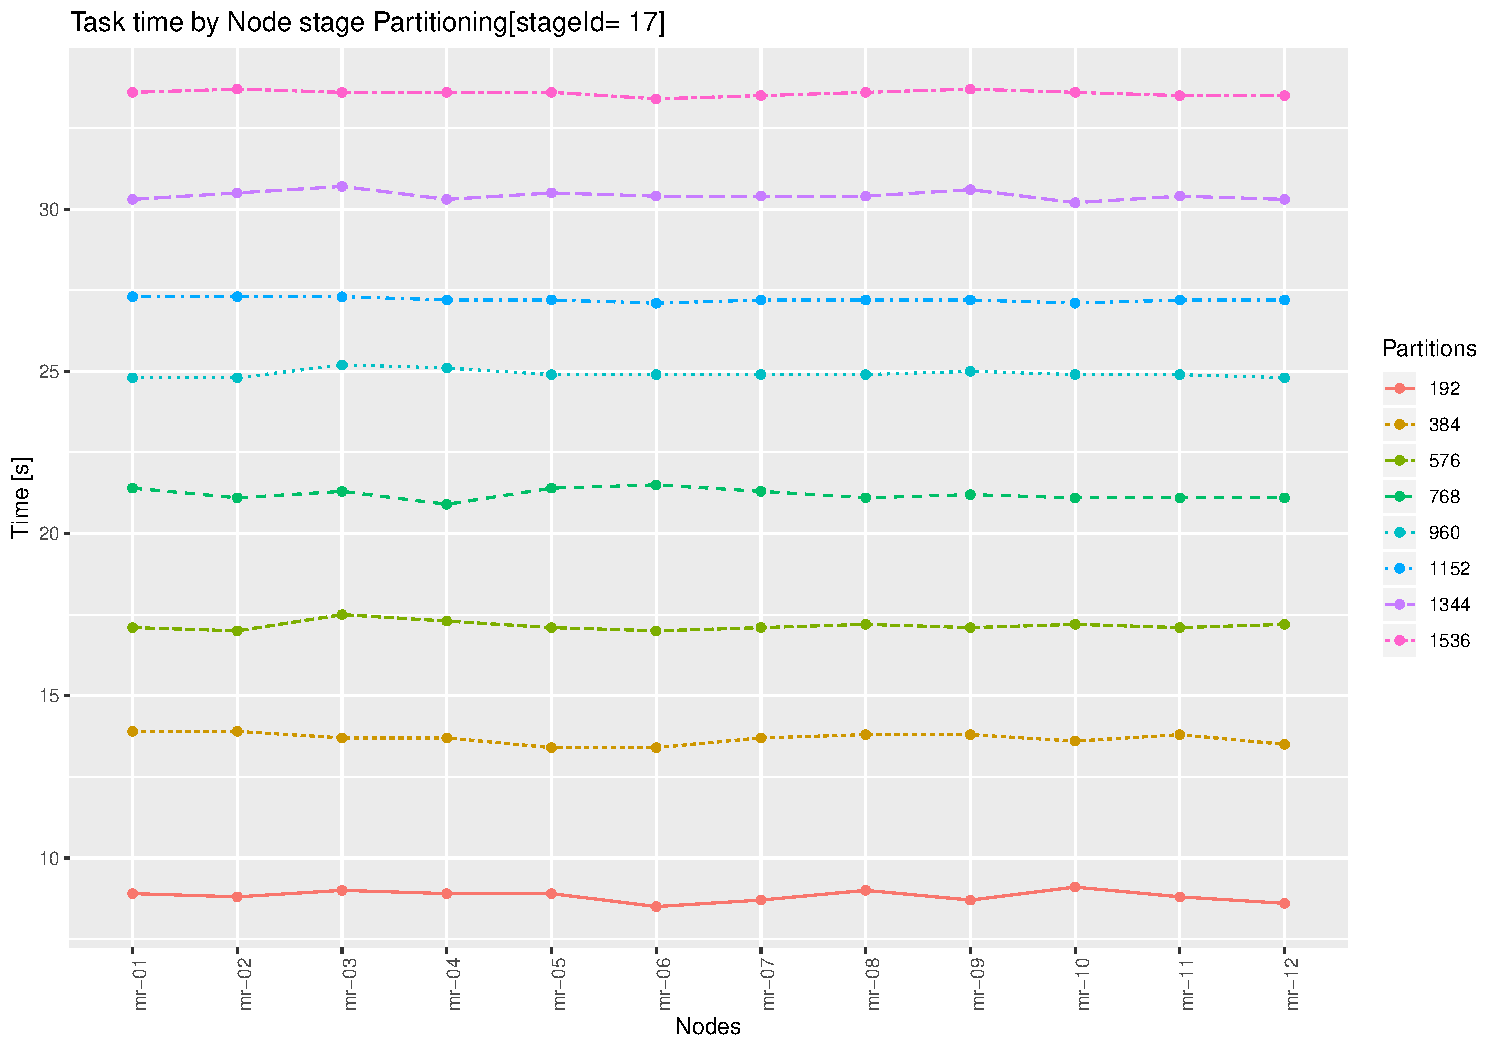
\includegraphics[width=0.85\textwidth]{figures/S17_Partitioning}
\end{frame}
\begin{frame}{Traking task balance in the cluster}
    \centering
	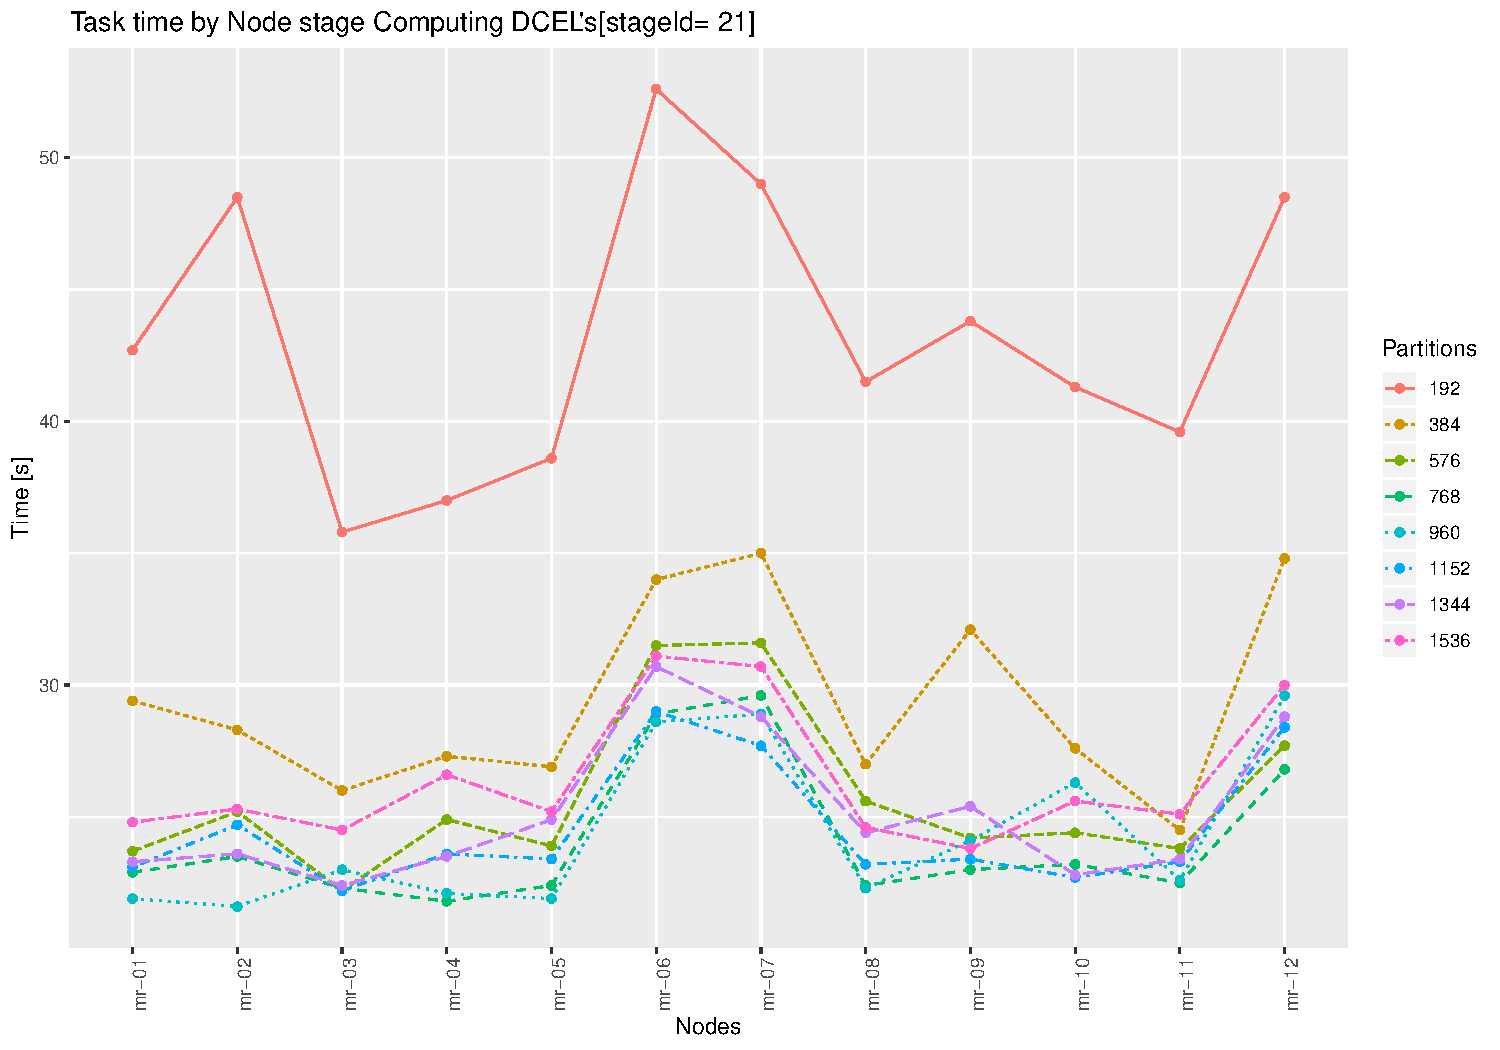
\includegraphics[width=0.85\textwidth]{figures/S21_ComputingDCEL}
\end{frame}
\begin{frame}{Traking task balance in the cluster}
    \centering
	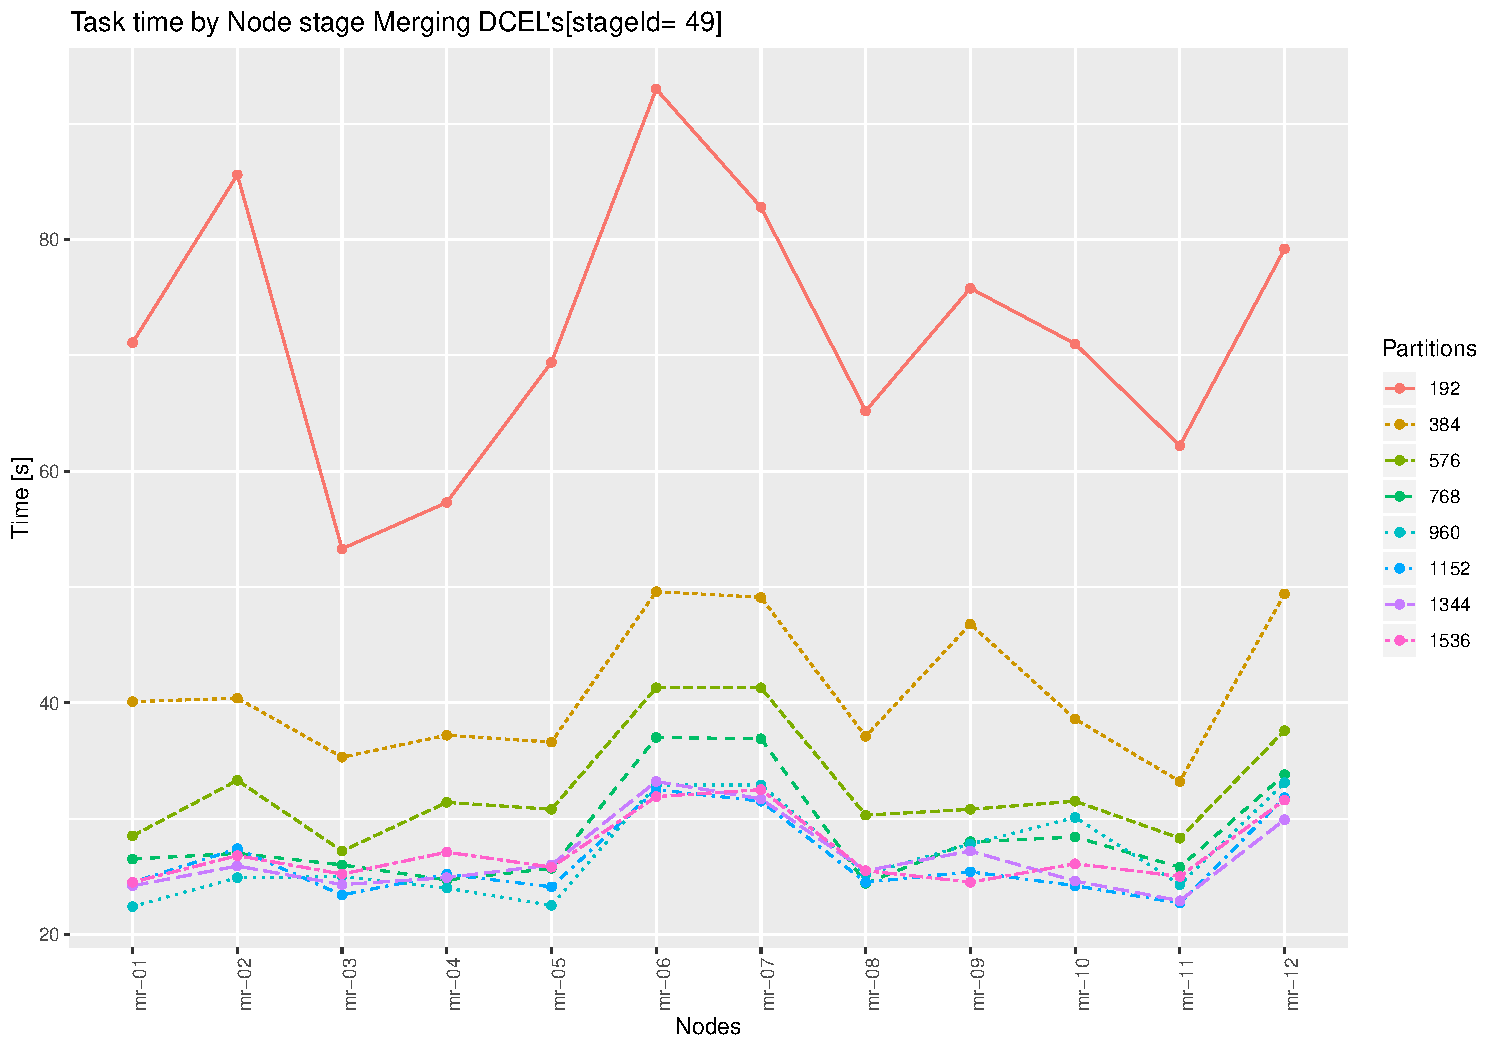
\includegraphics[width=0.85\textwidth]{figures/S49_MergingDCEL}
\end{frame}
\begin{frame}{Traking task balance in the cluster}
    \centering
	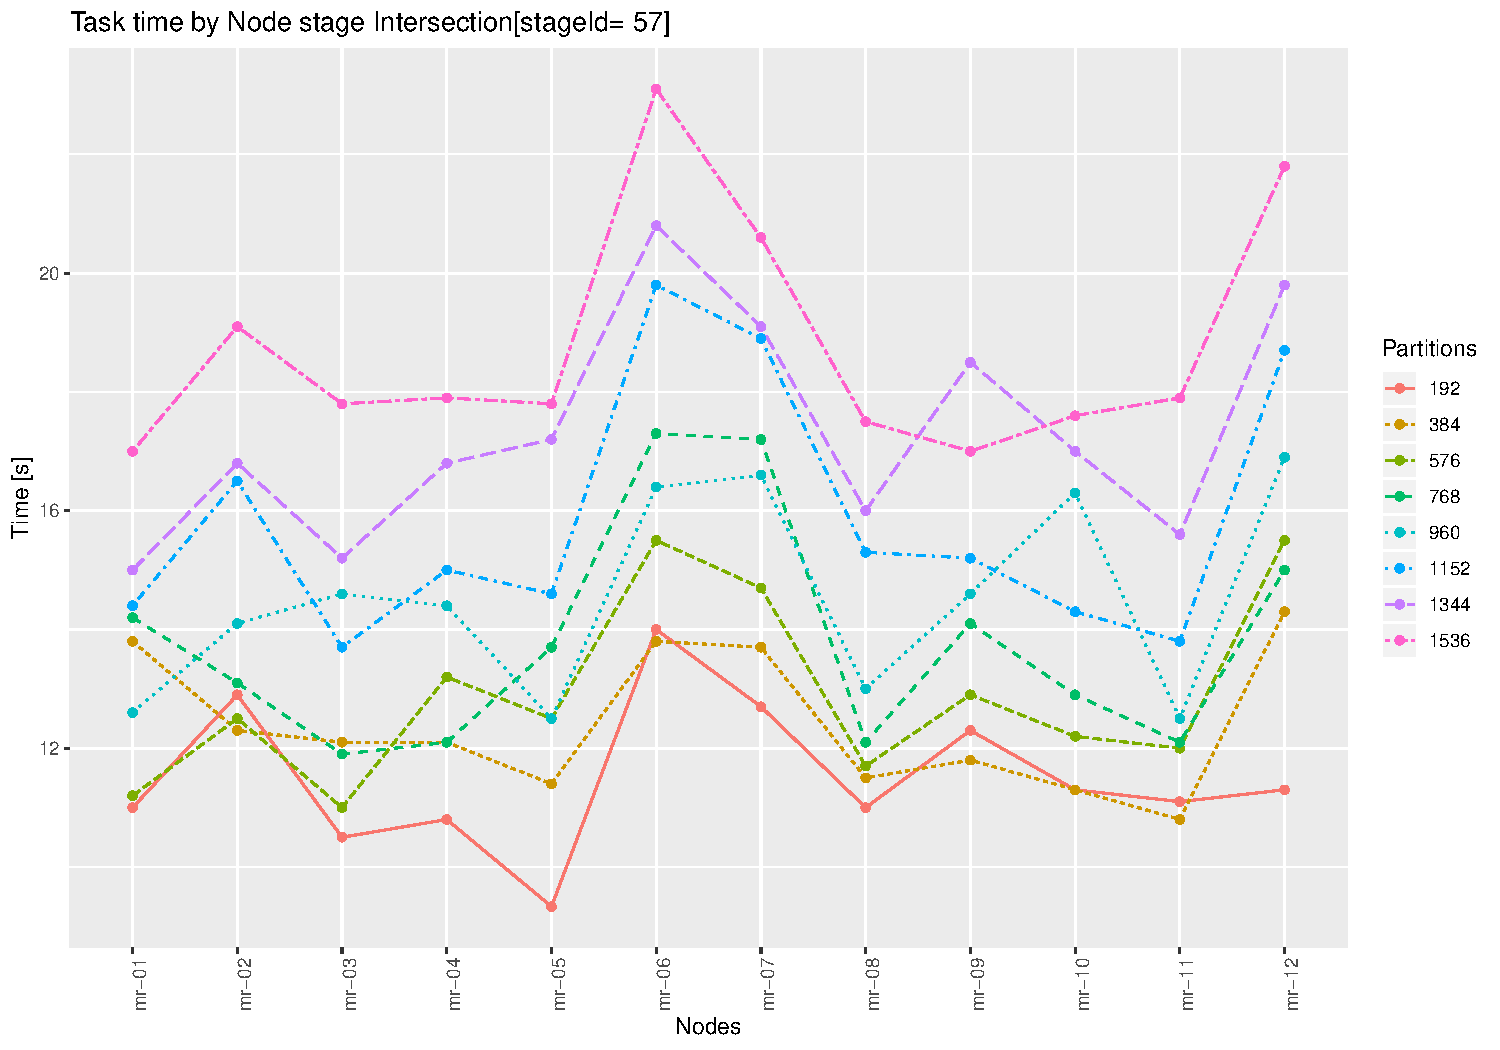
\includegraphics[width=0.85\textwidth]{figures/S57_Intersection}
\end{frame}

\end{document}
